%%%%%   INTRODUCCIÓN   %%%%%
%---------------------------------------------------------
%\section{Objetivo del documento}
%    El presente documento \varCveDocumento\ tiene como objetivo mostrar en detalle los requerimientos funcionales y no funcionales, modelos de información, reglas de negocio, modelos de comportamiento, casos de uso e interfaces correspondientes a cada uno de los módulos propuestos para esta etapa.

\section{Planteamiento del problema}
De acuerdo con la Organización para la Cooperación y el Desarrollo Económicos (OCDE), México tiene 2.2 médicos practicantes y 2.6 enfermeras practicantes por cada 1,000 habitantes, mucho menos que los promedios de la OCDE de 3.3 y 9.1 respectivamente. El número de camas hospitalarias también es considerablemente bajo, con 1.6 camas por cada 1,000 habitantes, comparado con 4.8 camas por cada 1,000 de la OCDE; siendo de los promedios más bajos dentro de los países que conforman la OCDE[1]. Aunado a esto, existe una gran demanda de atención médica y con los pocos espacios disponibles el servicio ofrecido se vuelve lento e ineficiente.\\

En consecuencia, existe una necesidad urgente de utilizar la tecnología para monitorear, informar y analizar de manera remota los signos vitales del paciente sin la necesidad de acudir con el personal médico. Esta forma de monitoreo beneficia tanto al paciente como a los hospitales pues se podrán tener registros de las mediciones de los signos en cualquier momento sin interrumpir la vida cotidiana del paciente y se tendrá la seguridad de que en una emergencia se podrá contactar a los familiares del paciente o a un médico para tratar la condición a tiempo.\\

\section{Solución propuesta}
Por lo anterior, hemos decidido crear un sistema que facilite el monitoreo remoto de la frecuencia cardíaca y de la temperatura corporal, que permita realizar las mediciones en cualquier momento utilizando un sensor específico para cada uno de los signos vitales mencionados anteriormente y con los datos medidos informar a personas interesadas, como familiares o médicos, del estado fisiológico del paciente que use el sistema y en caso de obtenerse valores anormales, tratar la emergencia lo más rápido posible.

\section{Justificación}
La tecnología se ha visto incorporada en prácticamente todas nuestras actividades cotidianas, como en el área de la salud o e-Salud, donde el uso de las tecnologías de información y comunicación (TIC) ha permitido la integración de los dispositivos para la medición remota y el registro preciso de los signos vitales, los cuales proporcionan una indicación del estado fisiológico de un paciente.\\

Una de las enfermedades a las que se les puede dar seguimiento mediante el monitoreo remoto son las enfermedades cardíacas y vasculares, o cardiovasculares, que son un grupo de desórdenes del corazón y de los vasos sanguíneos que incluyen afecciones tales como arritmias, enfermedad coronaria, ataque cardíaco, presión arterial alta, defectos cardíacos congénitos, demencia vascular y accidente cerebrovascular. Dichas enfermedades son la principal causa de muerte en todo el mundo  [8].  Tan solo en México, en el año 2016, se registraron 136,342 defunciones a causa de enfermedades del corazón, siendo también la primer causa de muerte en México [9].\\

La temperatura corporal también es un factor importante que se debe considerar con las personas que sufren algún trastorno de la regulación de la temperatura y al no requerir algún equipo de medición especializado, es también factible que se realice un monitoreo remoto de la misma, para detectar ciertas patologías por incremento o decremento de la temperatura corporal, que pueden provocar síndromes denominados menores o leves y cuadros clínicos mayores que pueden comprometer la vida del paciente [10].\\

Lo que se busca con este Trabajo Terminal es crear un sistema que permita capturar y enviar mediciones de la frecuencia cardíaca y la temperatura corporal de los pacientes que padezcan enfermedades a las que se les pueda dar seguimiento mediante el monitoreo remoto de estos signos vitales.\\

La propuesta comprenderá un dispositivo electrónico inalámbrico con un sensor para detectar el pulso cardíaco y uno para medir la temperatura corporal que permitirá la monitorización continua mediante la recopilación y procesamiento de la frecuencia cardíaca y la temperatura de la piel, que serán enviados al dispositivo móvil de las personas interesadas, como médicos y familiares.

\section{Objetivos}
\subsection{Objetivo general}
Implementar un sistema embebido que permita el monitoreo remoto de signos vitales de frecuencia cardíaca y temperatura corporal usando IoT.
\subsection{Objetivos específicos}
	\begin{itemize}
		\item Realizar la configuración y adquisición del sensor de pulso.
		\item Realizar la configuración y adquisición del sensor de temperatura.
		\item Realizar la configuración del módulo de comunicación entre el sistema y el teléfono celular.
		\item Diseñar y construir una aplicación móvil para la consulta de los valores enviados al teléfono celular.
		\item Diseñar y construir un sistema embebido para la medición y procesamiento del ritmo cardíaco.
	\end{itemize}	

\section{Productos o resultados esperados}
\textbf{Esta sección está en el protocolo pero no nos la dijo el profesor. ¿La dejamos?}

En la Figura \ref{fig:IntroduccionArqui} se muestra la arquitectura del sistema, la cual se conforma de cuatro etapas las cuales se describen a continuación:

\begin{enumerate}
	\item \textbf{Sensores.} En esta etapa se tomarán las mediciones de los signos vitales  con los sensores determinados durante el análisis.
	\item \textbf{Digitalización.} Una vez obtenidas las mediciones de los sensores, éstas pasarán a ser digitalizadas mediante un dispositivo digital programable para obtener la señal procesada.
	\item \textbf{Envío de datos.} Con los datos obtenidos en la etapa anterior, se realizará el envío a un teléfono celular.
	\item \textbf{Recepción de datos.}  Las señales procesadas de los signos vitales serán recibidas en el teléfono celular en donde se guardará el historial de los datos para futuras consultas.
\end{enumerate}

De la realización de este Trabajo Terminal se obtendrán los siguientes productos:

\begin{enumerate}
	\item Código.
	\item Sistema embebido.
	\item Aplicación móvil.
	\item Documentación técnica del sistema.
	\item Manual de usuario.
\end{enumerate}

\begin{figure}[htbp!]
	\centering
	\fbox{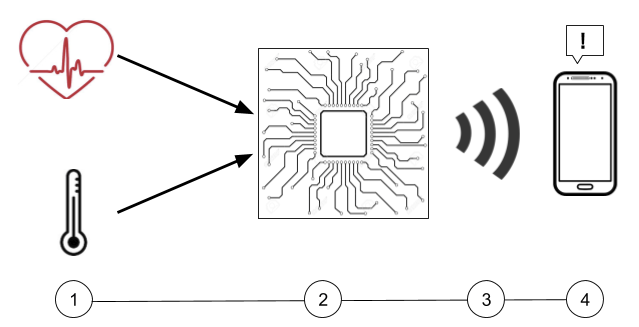
\includegraphics[width=0.8\textwidth]{images/introduccion/arquitectura.png}}
	\caption{Arquitectura del sistema.}
	\label{fig:IntroduccionArqui}
\end{figure}

\section{Metodología}
Para la realización del trabajo terminal se propone emplear el Modelo en V ya que ofrece una visión detallada de los diversos pasos e interacciones relacionados con el proceso de desarrollo y puede considerarse como un flujo de trabajo comúnmente utilizado. En la Figura \ref{fig:IntroduccionMetodologia} se muestran las principales actividades abordadas por el método. Convencionalmente, el lado izquierdo del modelo representa las fases del diseño del sistema, mientras que el lado derecho representa las fases de validación y verificación del sistema integrado.

\TODO \textbf{Cambiar resolución de imagen.}
\begin{figure}[htbp!]
	\centering
	\fbox{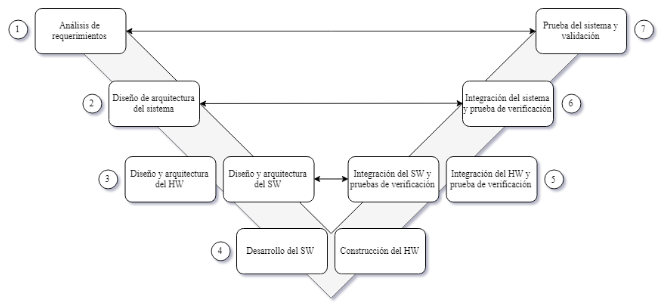
\includegraphics[width=\textwidth]{images/introduccion/metodologia.png}}
	\caption{Fases del modelo en V.}
	\label{fig:IntroduccionMetodologia}
\end{figure}

El desarrollo se llevará a cabo en las siguientes etapas:

\begin{enumerate}
	\item Análisis de requerimientos. Esta fase consiste en establecer qué debe hacer el sistema ideal, sin determinar cómo se construirá o diseñará el software. 
	\item Diseño de arquitectura del sistema. El diseño de la arquitectura del sistema consiste en varios pasos, como refinar las funciones del sistema y asignarlas a los diferentes componentes del sistema que pueden ser físicos o de hardware.
	\item Diseño de arquitectura de SW y HW. En esta fase del desarrollo del sistema, se diseña el hardware y el software de los diversos elementos que constituyen los componentes del sistema global. Las actividades que se aplican son similares a las realizadas en la fase anterior, pero centrándose en un componente específico del sistema: 
		\begin{itemize}
			\item Refinamiento de los requerimientos funcionales y no funcionales del hardware y software.
			\item Asignación de las funciones del software a los componentes de hardware.
		\end{itemize}
	\item Desarrollo del SW y Construcción del HW. Una vez que todos los componentes del sistema están diseñados, los elementos de hardware se construyen físicamente y los módulos de software son desarrollados en paralelo, y finalmente integrados con el hardware. Al final de este paso, los elementos de software y hardware deben estar disponibles para las actividades de verificación. Pueden realizarse algunas pruebas unitarias en paralelo con la implementación.
	\item Integración y verificación del SW y HW. En este paso se ensamblan los componentes de hardware y software. Las pruebas de verificación se ejecutan para comprobar el cumplimiento de los objetivos de diseño.
	\item Integración del sistema y prueba de verificación. En este paso, los elementos del sistema (HW, SW) se combinan y tiene lugar la verificación de los requisitos del sistema. 
	\item Prueba del sistema y validación. Esta última de verificación tiene como objetivo validar si los resultados obtenidos cumplen con los requerimientos.
\end{enumerate}

\section{Estructura del documento}
	\textbf{Creo que estaría bien agregar la descripción de los capítulos que abarca el documento pero no sé si aquí esté bien.}